\documentclass[10pt]{beamer}
\usetheme{Boadilla}

\usepackage{hyperref}
\usepackage{graphicx}
\usepackage{subfig}
\usepackage{amsmath,amssymb}

\graphicspath{ {images/} }

\usepackage{tikz}

%Some useful commands for QM
\newcommand{\bra}[1]{\left< #1 \right|}
\newcommand{\ket}[1]{\left| #1 \right>}
\newcommand{\expVal}[1]{\left< #1 \right>}
\newcommand{\braket}[2]{\left<#1|#2\right>}

%Stolen from http://tex.stackexchange.com/questions/178800/creating-sections-each-with-title-pages-in-beamers-slides
\AtBeginSection[]{
  \begin{frame}
  \vfill
  \centering
  \begin{beamercolorbox}[sep=8pt,center,shadow=true,rounded=true]{title}
    \usebeamerfont{title}\insertsectionhead\par%
  \end{beamercolorbox}
  \vfill
  \end{frame}
}

\title{Holographic Complexity in Non-Commutative Gauge Theory}
\subtitle{arxiv:1710.xxxxx, work with Stefan Eccles, Willy Fischler, and Ming-Lei Xiao}
\author{Josiah Couch}
\institute{University of Texas at Austin}
\date{20 Oct 2017}



\begin{document}

\begin{frame}
\titlepage\end{frame}

%\begin{frame}
%\frametitle{Outline}
%\tableofcontents[]
%\end{frame}

%\begin{frame}
%\frametitle{Introduction}

%Given the interest in recent years in holographic complexity, it is interesting to test the holographic conjectures in new settings. One potentially interesting setting is that of non-commutative field theory, where non-locality has been shown to have many interesting effects. We present a heuristic argument that one should expect an increase in the rate of growth of the state complexity as one makes a theory more non-commutative and test the complexity = action conjecture against this intuition for a family of holographic non-commutative field theories. We find that in the cases studied, as one increases the Moyal scale, the late time complexification rate is non-decreasing and in some cases we do see a sizeable increase.

%\end{frame}

\begin{frame}
\frametitle{Quantum Circuit Complexity}

\begin{itemize}

\item Consider a Hilbert space $\mathcal{H}$, e.g., the Hilbert space for $N$ quantum bits.

\item A universal gate set $\{g_i\}$ for $\mathcal{H}$ is a set of unitary operators on the Hilbert space such that any unitary $U$ acting on $\mathcal{H}$ can be approximated by some product $\displaystyle\prod_{i} g_{\alpha_i}$ to within a small tolerance $\epsilon$. 

\item Such a product of gates is referred to as a quantum circuit.

\item The quantum circuit complexity of a unitary $U$ is then the minimum number of gates needed to approximate $U$ to within the tolerance.

\item In the example of qubits, one typically considers gates that act on a single qubit or pairs of qubits at a time.

\item Given some reference state $\ket{\psi_R}$, one may define the complexity of a state $\ket{\psi}$ as the minimum of complexity $C(U)$ over all unitaries $U$ such that $\ket{\psi} = U\ket{\psi_R}$.

\end{itemize}

\end{frame}

\begin{frame}
\frametitle{Holographic Complexity}

\begin{itemize}

\item So far there are at least three proposals for the holographic dual of the complexity of the state of the boundary field theory. The proposed duals are the volume of a maximal spatial slice ('complexity = volume'), the action evaluated on a Wheeler-DeWitt (WDW) patch ('complexity = action'), and the spacetime volume of a WDW patch ('complexity = spacetime volume'). 

\item These proposals are motivated by the late time behavior of the volume of a two-sided black hole

\item All three proposals involve different measures of the 'size' of a black hole

\item One piece of evidence for these conjectures is that they exhibit the correct behavior for precursor operators, which measure the difference between the state now, and what state we would have now had we inserted an operator $\mathcal{O}$ at an earlier time $t$. 

\item For this work we have focused on the complexity = action conjecture. 

\end{itemize}

\end{frame}



\begin{frame}
\frametitle{Action on a WDW patch}

\begin{figure}
    \begin{center}
    
        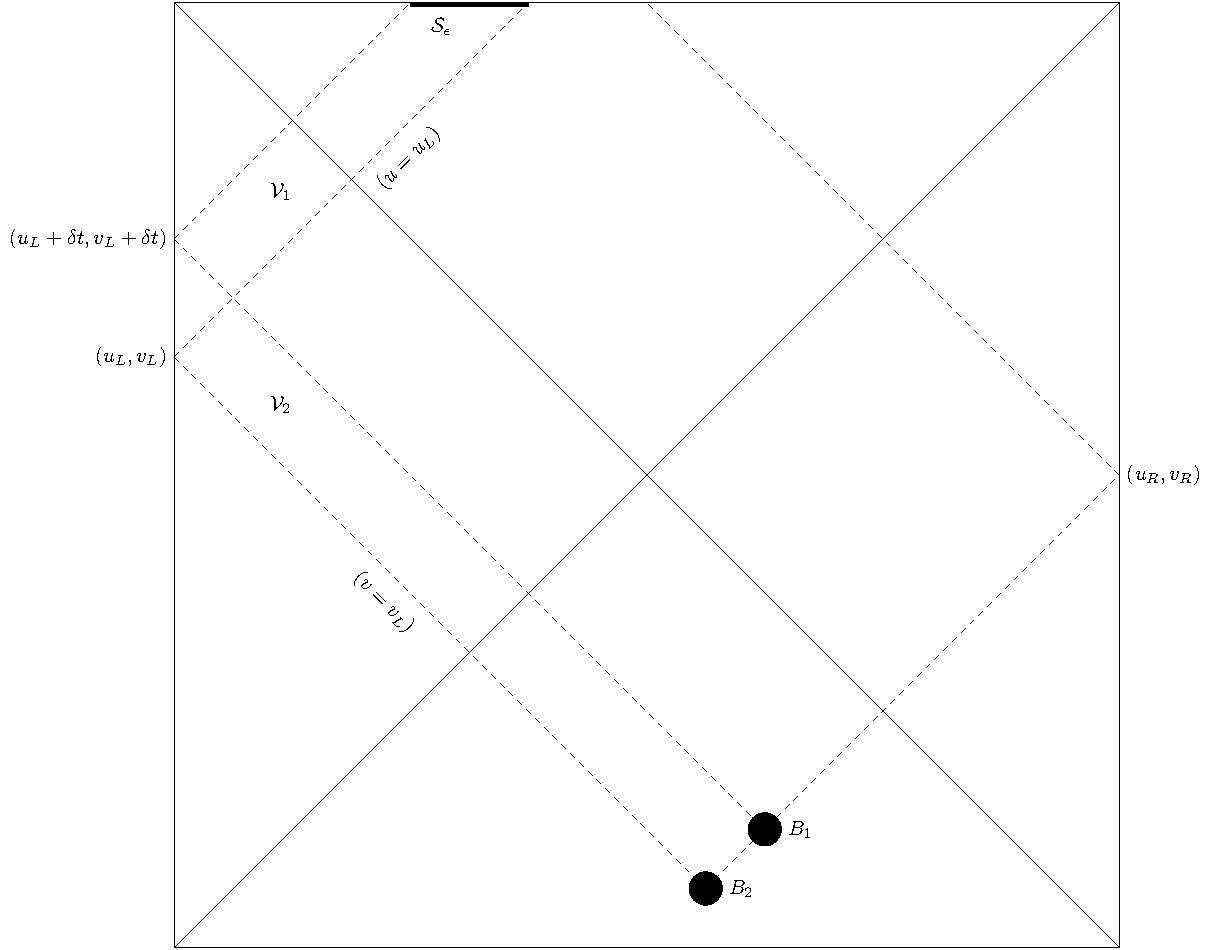
\includegraphics[scale=0.5]{WDW.pdf}    
    
    \end{center}
    \caption{Two WDW patches separated by $\delta t$.  Although the boundary of each patch is really at some large but finite $r_b$, the choice of $r_b$ drops out in the differences we consider and we do not indicate it explicitly in this graphic.}
    \label{fig:WDW}
\end{figure}

\end{frame}


\begin{frame}
\frametitle{Non-Commutative SYM}

\begin{itemize}

\item We would like to test complexity = action in a new context. However, computing the complexity of a state in a strongly couped field theory is not something we know how to do. Instead, we will rely on our intuition about the qualitative behavior of complexity in some novel situation.

\item A good candidate is SYM living on a non-commutative geometry, i.e., a geometry where two of the spatial directions don't commute.

\item A gravity dual to such a theory was derived in the late 90's by a number of authors \cite{Hashimoto:1999ut, Maldacena:1999mh}.

\item Generalizations of this system to other numbers of dimensions have also been considered in, e.g., \cite{Alishahiha:1999ci, Berman:2000jw}.

\item These solutions are obtained by considering a stack of Dp-branes in type II string theory and exciting a compenent of the NS-NS 2-form B-field along two of the worldsheet directions.

\item Additional non-commutativities can be introduced by turning on additional complenets of the B-field.

\end{itemize}

\end{frame}\begin{frame}
\frametitle{Non-Commutativity and Complexity: A heuristic argument}

\begin{figure}
    \begin{center}
        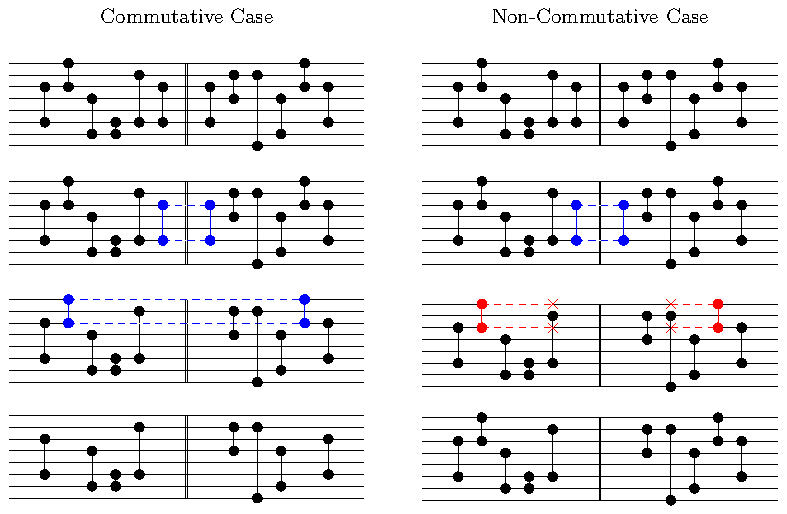
\includegraphics[scale=0.6]{cartoon}
    \end{center}
   \caption{Consider an optimal circuit that evolves our state by a small time $\delta t$. As we compose this circuit many times, we expect some cancelations between gates in adjacent copies of the ciruit. Non-commutativity acts as an impediment to such cancelation by making fewer gates commute (due to non-locality), and so the final ciruit after cancelation is more complex.} \label{fig:cartoon1}
\end{figure}

\end{frame}


\begin{frame}
\frametitle{Our Results}

\begin{figure}[htbp]
    \begin{center}
        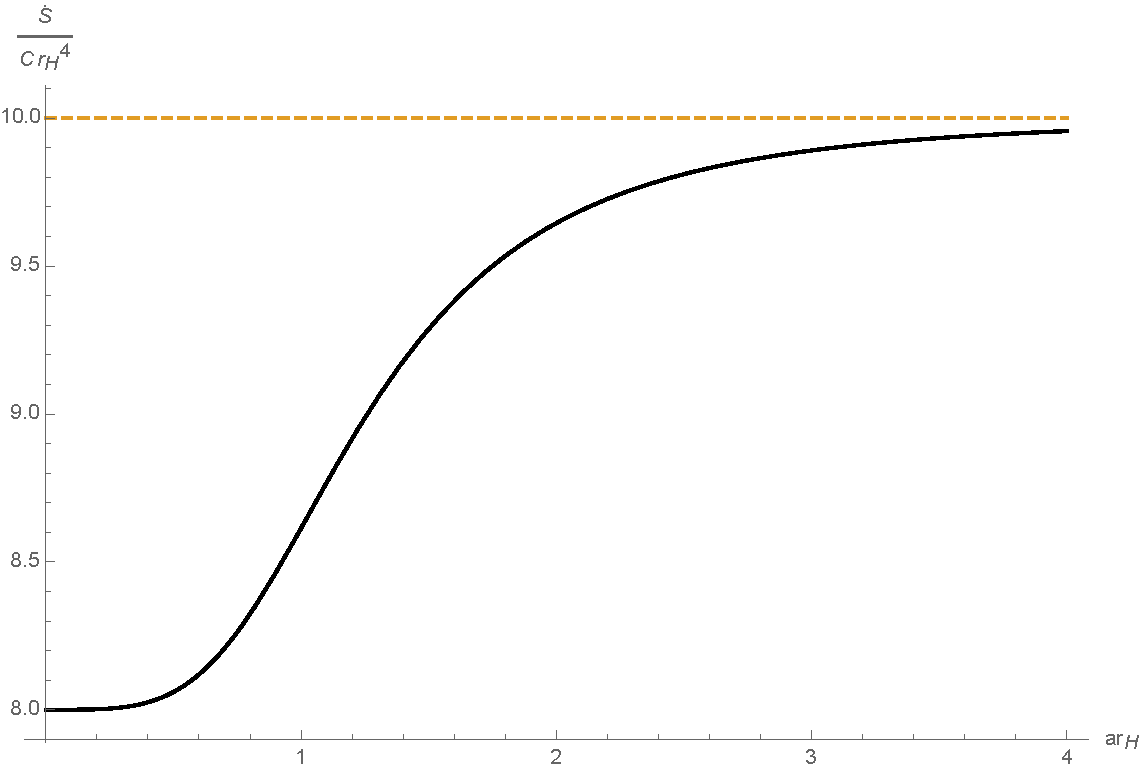
\includegraphics[scale=0.3]{LateTime}
    \end{center}
    \caption{Late time action growth rate normalized by $C=\frac{\alpha^4 \Omega_5 V_3}{\hat{g}_s^2}$ and extra $r_H$ dependence, versus $a r_H$, which is the Moyal scale measured in units of thermal length.} 
    \label{fig:LateTime}
\end{figure}

\begin{table}
    \centering
    \begin{tabular}{l | c  c  c }
        $p$ & $m=0$ & $m=1$ & $m=2$ \\
        \hline
        2 & 12 & 12 & - \\
        3 & 8 & 10 & - \\
        4 & 5 & 5 & 8 \\
        5 & 4 & 5 & 6 \\
    \end{tabular}
\end{table}

\end{frame}

\begin{frame}
\frametitle{Conclusions}

\begin{itemize}

\item For $p=3,5$ we do see an increase, as expected.

\item Though we did not see an increase for $p=2$ or for $p=4$ with a single non-trivial commutator, we did not see a decrease either.

\item Overall, the results are consistent with the heuristic argument above.

\item This result is in tension with the idea that commutative black holes are he fastest possible computers

\item In future work we plan to repeat our calculations for complexity = volume.

\end{itemize}

\end{frame}

\begin{frame}
\frametitle{References}

\bibliographystyle{JHEP} %JHEP.bst
\footnotesize\bibliography{NCG} %NCG.bib

\end{frame}

\end{document}